% В этом документе преамбула

\documentclass[a4paper,12pt]{article}

\usepackage{lscape} % горизонтальный режим
\usepackage{pdflscape}

\usepackage{lipsum} % тестовые тексты

%%% Работа с русским языком
\usepackage{cmap}					% поиск в PDF
\usepackage{mathtext} 				% русские буквы в формулах
\usepackage[T2A]{fontenc}			% кодировка
\usepackage[utf8]{inputenc}			% кодировка исходного текста
\usepackage[english,russian]{babel}	% локализация и переносы
\usepackage{indentfirst}			% чтобы первый абзац в разделе отбивался красной строкой
\frenchspacing						% тонкая настройка пробелов
\usepackage{gensymb}				% символы по типу градусов
\usepackage{algorithm}				% для алгоритмов
\usepackage{algorithmic}			% для алгоритмов

%%% Приведение начертания букв и знаков к русской типографской традиции
\renewcommand{\epsilon}{\ensuremath{\varepsilon}}
\renewcommand{\phi}{\ensuremath{\varphi}}			% буквы "эпсилон"
\renewcommand{\kappa}{\ensuremath{\varkappa}}		% буквы "каппа"
\renewcommand{\le}{\ensuremath{\leqslant}}			% знак меньше или равно
\renewcommand{\leq}{\ensuremath{\leqslant}}			% знак меньше или равно
\renewcommand{\ge}{\ensuremath{\geqslant}}			% знак больше или равно
\renewcommand{\geq}{\ensuremath{\geqslant}}			% знак больше или равно
\renewcommand{\emptyset}{\varnothing}				% знак пустого множества

%%% Дополнительная работа с математикой
\usepackage{amsmath,amsfonts,amssymb,amsthm,mathtools,esint} % AMS
\usepackage{wasysym}
\usepackage{icomma} % "Умная" запятая: $0,2$ --- число, $0, 2$ --- перечисление

%% Номера формул
\mathtoolsset{showonlyrefs=true} % Показывать номера только у тех формул, на которые есть \eqref{} в тексте.

%% Свои команды

% операции, не определённые (или имеющие иные обохначения) в мат. пакетах
\DeclareMathOperator{\sgn}{\mathop{sgn}}				% ф-ия sgn
\renewcommand{\tg}{\mathop{\mathrm{tg}}\nolimits}		% обозначение тангенса

%% Перенос знаков в формулах (по Львовскому)
\newcommand*{\hm}[1]{#1\nobreak\discretionary{}
{\hbox{$\mathsurround=0pt #1$}}{}}

%%% Работа с картинками
\usepackage{graphicx}  				% Для вставки рисунков
\graphicspath{{images/}{images2/}}  % папки с картинками
\setlength\fboxsep{3pt} 			% Отступ рамки \fbox{} от рисунка
\setlength\fboxrule{1pt} 			% Толщина линий рамки \fbox{}
\usepackage{wrapfig} 				% Обтекание рисунков текстом

%%% Работа с таблицами
\usepackage{array,tabularx,tabulary,booktabs} 	% Дополнительная работа с таблицами
\usepackage{longtable}  						% Длинные таблицы
\usepackage{multirow}							% Слияние строк в таблице

%%% Теоремы

\newtheoremstyle{break}% name
	{}%         Space above, empty = `usual value'
	{}%         Space below
	{\itshape}% Body font
	{}%         Indent amount (empty = no indent, \parindent = para indent)
	{\bfseries}% Thm head font
	{.}%        Punctuation after thm head
	{\newline}% Space after thm head: \newline = linebreak
	{}%         Thm head spec
\theoremstyle{break}

% \theoremstyle{plain} % Стиль по умолчанию
\newtheorem{theorem}{Теорема}[section]
\newtheorem{lemma}{Лемма}[section]
\newtheorem{definition}[theorem]{Определение}
\newtheorem{property}{Свойство}
 
\newtheorem{corollary}{Следствие}[theorem]

\newtheoremstyle{example}	% style name
	{2ex}					% above space
	{2ex}					% below space
	{}						% body font
	{}						% indent amount
	{\bf}				% head font
	{.}						% post head punctuation
	{\newline}				% post head punctuation
	{\thmname{#1}\thmnumber{ #2}\thmnote{ (#3)}}						% head spec

\theoremstyle{example}
\newtheorem{exmp}{Пример}[section]
 
\theoremstyle{remark} % "Примечание"
\newtheorem*{nonum}{Решение}
\newtheorem*{evidence}{Доказательство}
\newtheorem*{remark}{Примечание}

%%% Программирование
\usepackage{etoolbox} % логические операторы

%%% Страница
\usepackage{extsizes} % Возможность сделать 14-й шрифт
\usepackage{geometry} % Простой способ задавать поля
	\geometry{top=15mm}
	\geometry{bottom=35mm}
	\geometry{left=10mm}
	\geometry{right=10mm}

%\usepackage{fancyhdr} % Колонтитулы
% 	\pagestyle{fancy}
 	%\renewcommand{\headrulewidth}{0pt}  % Толщина линейки, отчеркивающей верхний колонтитул
% 	\lfoot{Нижний левый}
% 	\rfoot{Нижний правый}
% 	\rhead{Верхний правый}
% 	\chead{Верхний в центре}
% 	\lhead{Верхний левый}
%	\cfoot{Нижний в центре} % По умолчанию здесь номер страницы

\usepackage{setspace} % Интерлиньяж (межстрочные интервалы)
%\onehalfspacing % Интерлиньяж 1.5
%\doublespacing % Интерлиньяж 2
%\singlespacing % Интерлиньяж 1

\usepackage{lastpage} % Узнать, сколько всего страниц в документе.

\usepackage{soulutf8} % Модификаторы начертания

\usepackage{hyperref}
\usepackage[usenames,dvipsnames,svgnames,table,rgb]{xcolor}
\hypersetup{				% Гиперссылки
    unicode=true,           % русские буквы в раздела PDF
    pdftitle={Заголовок},   % Заголовок
    pdfauthor={Автор},      % Автор
    pdfsubject={Тема},      % Тема
    pdfcreator={Создатель}, % Создатель
    pdfproducer={Производитель}, % Производитель
    pdfkeywords={keyword1} {key2} {key3}, % Ключевые слова
    colorlinks=true,       	% false: ссылки в рамках; true: цветные ссылки
    linkcolor=MidnightBlue, % внутренние ссылки
    citecolor=black,        % на библиографию
    filecolor=magenta,      % на файлы
    urlcolor=blue           % на URL
}

\usepackage{csquotes} % Еще инструменты для ссылок

%\usepackage[style=authoryear,maxcitenames=2,backend=biber,sorting=nty]{biblatex}

\usepackage{multicol} % Несколько колонок

%%% Работа с графикой
\usepackage{tikz}
\usetikzlibrary{calc}
\usepackage{tkz-euclide}
\usetikzlibrary{arrows}
\usepackage{pgfplots}
\usepackage{pgfplotstable}

%%% Настройка подписей к плавающим объектам
% \usepackage{floatrow}	% размещение
\usepackage{caption}	% начертание
\captionsetup[figure]{labelfont=bf,textfont=it,font=footnotesize}	% нумерация и надпись курсивом
% для подфигур: заголовок подписи полужирный, текст заголовка обычный
% выравнивание является неровным (т.е. выровненным по левому краю)
% singlelinecheck = off означает, что настройка выравнивания используется, даже если заголовок имеет длину только одну строку.
% если singlelinecheck = on, то заголовок всегда центрируется, когда заголовок состоит только из одной строки.
\captionsetup[subfigure]{labelfont=bf,textfont=normalfont,singlelinecheck=off,justification=raggedright}

%%% Stuff для листинга
\usepackage{listings}
\usepackage{xcolor}

\colorlet{mygray}{black!30}
\colorlet{mygreen}{green!60!blue}
\colorlet{mymauve}{red!60!blue}

\lstset{
	backgroundcolor=\color{gray!10},  
	basicstyle=\ttfamily,
	columns=fullflexible,
	breakatwhitespace=false,      
	breaklines=true,                
	captionpos=b,                    
	commentstyle=\color{mygreen}, 
	extendedchars=true,              
	frame=single,                   
	keepspaces=true,             
	keywordstyle=\color{blue},      
	language=c++,                 
	numbers=none,                
	numbersep=5pt,                   
	numberstyle=\tiny\color{blue}, 
	rulecolor=\color{mygray},        
	showspaces=false,               
	showtabs=false,                 
	stepnumber=5,                  
	stringstyle=\color{mymauve},    
	tabsize=3,                      
	title=\lstname                
}

% для извращённых начертаний
\usepackage{mathrsfs}

\usepackage{makecell}
\setcellgapes{3pt}

% Зачёркивание символов
\usepackage{cancel}

% перечисления с буквами
\usepackage{enumitem}

\DeclareMathOperator{\eq}{\Leftrightarrow}

\begin{document} % начало документа

\textit{Лектор:} Толкачева Алёна Алексеевна

\begin{align}
	\textbf{06.02.2020}
\end{align}

\section{Основные алгебраические структуры}

\subsection{Функции, отображения множеств}

Пусть $A, B$ - множества. $A \times B = \{ (a,b) | a \in A, b \in B \}$

\begin{definition}[Функция]
	Подмножество $f$ декартова произведения называется \textbf{функцией}, если $\forall a \in A, b_1, b_2 \in B:$
	\[
		\left.
			\begin{aligned}
				(a, b_1) \in f \\
				(a, b_2) \in f
			\end{aligned}
		\right\}
		\Rightarrow b_1 = b_2
	\]
	
	Эквивалентная запись:
	\[ f \subseteq A \times B \text{ и } f: A \to B, \]
	\[ (a,b) \in f \text{ и } f(a) = b \]
\end{definition}

Функция - это НЕ соответствие (!), это подмножество декартового произведения, где каждому элемента из 1-ого множества ставится не более одного элемента из 2-ого.

\begin{definition}[Область определения]
	Областью определения функции $f \subseteq A \times B$ называется множество $D_f = \{a \in A | \exists b \in B: (a, b) \in f\}$
\end{definition}

\begin{definition}[Область значений]
	Областью значений функции $f \subseteq A \times B$ называется множеством $E_f = \{b \in B | \exists a \in A: (a, b) \in f\}$
\end{definition}

\begin{definition}
	Нечёткое множество: лысый человек, куча сена - с какого кол-ва волос / колосков можно считать лысым / стогом. С какой долей (весом) попадает в это множество.
\end{definition}

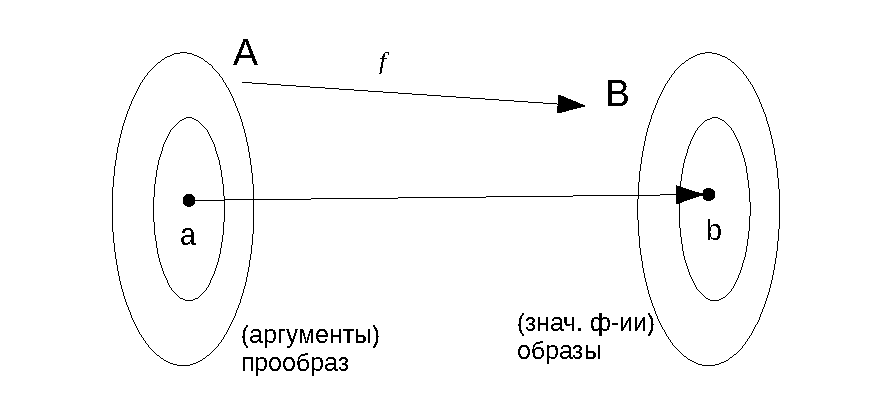
\includegraphics[scale=0.7]{./media/proobraz.pdf}

\begin{definition}[Отображения]
	Функция $f: A \to B$ называется отображением, если $\forall a \in A \exists ! b \in B: f(a) = b.$
\end{definition}

\begin{theorem}[Критерий отображения]
	Функция $f: A \to B$ явл-ся отображением ТТТ, когда $D_f = A$.
\end{theorem}

\begin{proof}
	Доказываем необходимость и достаточность.
	
	Дано: $f: A \to B$ - отображение.
	
	\underline{Необходимость:}
	
	\[ \forall a \in A \exists ! \underbrace{b \in B: f(a) = b}_{\text{по усл.}} \]
	\[
	\begin{cases}
		D_f \subseteq A (\text{по усл.}) \\
		A \subseteq \underbrace{D_f}_{a \in D_f}
	\end{cases}
	\Rightarrow D_f = A
	\]
	
	\underline{Достаточность:}
	
	Если $D_f = A$:
	\[ \forall a \in A = D_f \]
	\[ \exists b \in B: f(a) = b \]
	(!) по def функции.
\end{proof}

\begin{definition}
	Отображение $f: A \to A$ наз-ся преобразованием множества $A$.
\end{definition}

\textbf{Свойства функций:}

\begin{itemize}
	\item Функция $f: A \to B$ наз-ся \textbf{инъективной (инъекций)}, если $\forall a_1, a_2 \in A: a_1 \ne a_2 \Rightarrow f(a_1) \ne f(a_2)$.
	\item Отображение $f: A \to B$ называется \textbf{сюръективным (сюръекцией)}, если $\forall b \in B \exists a \in A: f(a) = b$ - для любого образа надётся прообраз.
	\item Отображене $f: A \to B$ называется \textbf{биективным (биекцией)}, если оно инъективно и сюръективно одновременно.
\end{itemize}

\begin{theorem}[Критерий сюръективности]
	\[ f: A \to B - \text{сюр.} \eq E_f = B \]
\end{theorem}

\textbf{Пример 1.}

\[ A = B = \mathbb{R} \]
\[ A \times B = \mathbb{R}^2 - \text{плоскость} \]

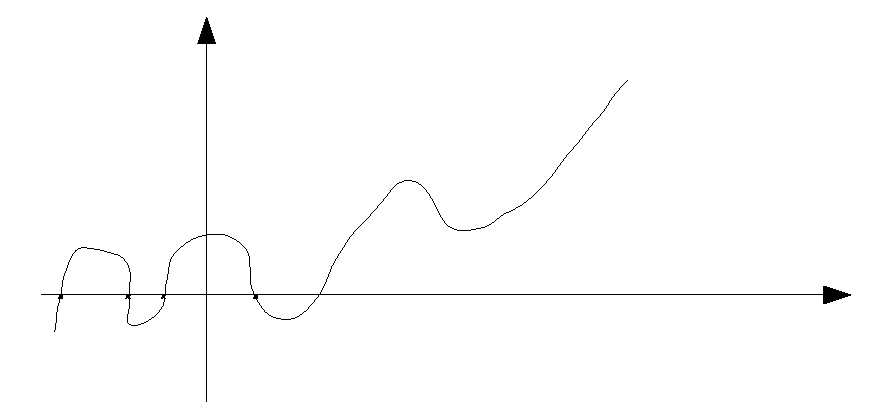
\includegraphics[]{./media/sur_ex_1.pdf}

Комплексные корни ходят сопряжёнными парами. 

Любая волна (см. 1-ую четверть) отвечает за пары корней.

Отображение - область определения - всё 1-ое множество. Здесь ф-ия уходит в бесконечность в обе стороны $\Rightarrow$ является отображением (мн-н определён везде).

Функция не инъективна, т.к. для разных значений есть одинаковые значения.

Т.к. не инъективна, значит не биективна.

Сюръективна, т.к. для любого образа найдётся свой прообраз.

~

\textbf{Пример 2. (Гардероб)}

Есть номерки - 1-ая группа людей, 2-ая группа - крючки. Функция: выбираем только те элементы, которые составляют пары куртка, повешанная на крючок. Что <<обрезать>>, чтобы получить нормальную ф-ию? Запретить вешать одну одежду на несколько крючков, а не на несколько $\Rightarrow$ возникает функциональная зависимость.

Наша функция станет отображением, когда не будет не повешенной одежды.

Станет сюръекцией, когда все крючки будут заняты.

$\Rightarrow$ устанавливает биективное отношение $\eq$ взаимное соответствие.

Если на крючках написать ещё номера (конечное $\{1,2,\dots,n\}$), то установим взаимооднозначное соответствие.

\subsection{Операции на множествах}

Пусть $A$ - множество.

\[ A^n = \{ (a_1, a_2, \dots, a_n) | a_i \in A, \forall i = \overline{1, n} \} \]

\begin{definition}
	Произвольное отображение $f: A^n \in A$ наз-ся $n$-арной алгебраической операцией (операцией, замкнутой на $A$).
	
	При $n = 2$ говорят о \textit{бинарных операциях}.
	
	\[ f(\underbrace{a_1, a_2,...,a_n}_{\in A^n}) = \underbrace{b}_{\in A} \]
	\[ f: \underbrace{\mathbb{R}}_{>0} \to \underbrace{\mathbb{R}}_{>0} \]
	\[ x \to e^{(x-1)} \]
\end{definition}

\begin{definition}
	Бинарная операция $f$ \textbf{замкнута} на множестве $A$ (алгебраическое действие), если
	\[ \forall a_1, a_2 \in A: f(a_1, a_2) \in A. \]
\end{definition}

Дано: $f(a_1, a_2) = b \sim ...$ если используем значок $+$ - используем \textbf{аддитивную запись}, если используем $\times$ или $\cdot$ - используем \textbf{мультипликативную запись}.

\textbf{Свойства алгебраических бинарных операций:}

\begin{itemize}
	\item Ассоциативность: $\forall a_1, a_2, a_3 \in A: (a_1 * a_2) * a_3 = a_1 * (a_2 * a_3)$
	\item Коммутативность: $\forall a_1, a_2 \in A: a_1 * a_2 = a_2 * a_1$
	\item Обратимость справа: $\forall a_1, a_2 \in A \exists x \in A: a_1 = a_2 * x$
	\item Обратимость слева: $\forall a_1, a_2 \in A \exists x \in A: a_1 = x * a_2$
	\item Сократимость справа: $\forall a_1, a_2, x \in A: a_1 * x = a_2 * x \Rightarrow a_1 = a_2$
	\item Сократимость слева: $\forall a_1, a_2, x \in A: x * a_1 = x * a_2 \Rightarrow a_1 = a_2$
\end{itemize}

Пусть на множестве $A$ введена бинарная операция $*$.

\begin{definition}
	Элемент $e$ множества $A$ называется \textbf{правой (левой) единицей}, если $\forall a \in A: a * e = a(e * a = a)$. 
\end{definition}

\begin{definition}
	Элемент называется \textbf{нейтральным (единицей)}, если он является и левой, и правой единицами.
\end{definition}

\begin{definition}
	Элемент $a \in A$ \textbf{обратим справа (слева)}, если $\exists a' \in A: a * a' = e(a' * a = e)$.
\end{definition}

\begin{definition}[Обратимость элемента]
	Элемент обратим, если он обратим и справа, и слева.
\end{definition}

\begin{exmp}
	\[ A = \{ a, b, c \}, *: x * \underbrace{y}_{\text{правая единица}} = x, \forall x, y \in A \]
	
	Таблица Кэли (таблица действий):
	
	\begin{table}[h]
		\centering
		\begin{tabular}{l|lll}
			$*$ & $a$ & $b$ & $c$ \\ \hline
			$a$ & $a$ & $a$ & $a$ \\
			$b$ & $b$ & $b$ & $b$ \\
			$c$ & $c$ & $c$ & $c$
		\end{tabular}
	\end{table}

	$\Rightarrow$ операция замкнута и ассоциативна.
	
	\begin{itemize}
		\item $x * (y * z) = x * y = x; (x * y) * z = x * z = x \Rightarrow$ не коммунитативна (иначе таблица Кэли должна быть симметрична)
		\item Каждый элемент является левым нулём и правой единицей: $\forall x \in A: x * a = x$ - все элементы правые единицы. Нулевой элемент всё вбирает в себя.
	\end{itemize}
\end{exmp}

\begin{definition}
	Элемент $\Theta$ множества $A$ называется правым (левым) нулём, если $\forall a \in A: a * \Theta = \Theta (\Theta a = \Theta)$.
\end{definition}

\begin{definition}
	Элемент является \textbf{нулевым (нулём)}, если он является и левым, и правым нулём.
	
	Каждый элемент иденпотентен (произведение на себя - даёт сам себя).
\end{definition}

\begin{definition}
	Элемент $a \in A$ - иденпотентен, если $a * a = a$.
\end{definition}

\begin{definition}
	Элемент $a \in A$ наз-ся нильпотентным, если $a * a = \Theta$.
\end{definition}

\begin{exmp}
	$M_{m \times n}$
	
	$E_{m \times m}$ - левая ед.
	
	$E_{n \times n}$ - правая ед.
\end{exmp}

\subsection{Алгебраические структуры}

\begin{definition}[Алгебраическая структура]
	Множество $A$, с введёнными на нём операциями $m$ алгебраическими (замкнутыми) операциями. наз-ся алгебраической структурой.
	\[ (A, *_1, *_2, \dots, *_m) \]
\end{definition}

\begin{definition}[Подструктура]
	Подструктурой называется непустое подмножество $A$, являющееся алгебраической структурой относительно наследуемых операций.
\end{definition}

\begin{exmp}
	$L$ - линейное пространство. Операции: $+$ - бинарная операция - сложение, $\lambda \cdot$ - унарная операция - умножение на число: $P \cdot \bar a \in L, P$ - числа. Получаем \textit{линейное пространство}. Операция должна сохраняться и на подпространстве.
\end{exmp}

\[ (A, *) \]

\begin{definition}
	Полугруппа - мн-во с одной замкнутой ассоциативной операцией. Полугруппа наз-ся \textbf{коммутативной}, если операция на ней коммунитативна. Полугруппа с единицей - \textbf{моноид}.
\end{definition}

\begin{definition}
	Группа - мн-во с одной замкнутой, ассоциативной, обратимой операцией. Группа наз-ся \textbf{коммутативной (абелевой) группой}, если операция на ней коммутативна.
\end{definition}

\[ K, +, \cdot - \text{кольцо, если} \]

\begin{itemize}
	\item $(K, +)$ - абелева группа
	\item $(K, \cdot)$ - полугруппа
	\item $\forall a, b, c \in K:$
	\[
	\begin{aligned}
		(a+b)c = ac + bc \\
		a(b+c) = ab + ac
	\end{aligned}
	\]
\end{itemize}

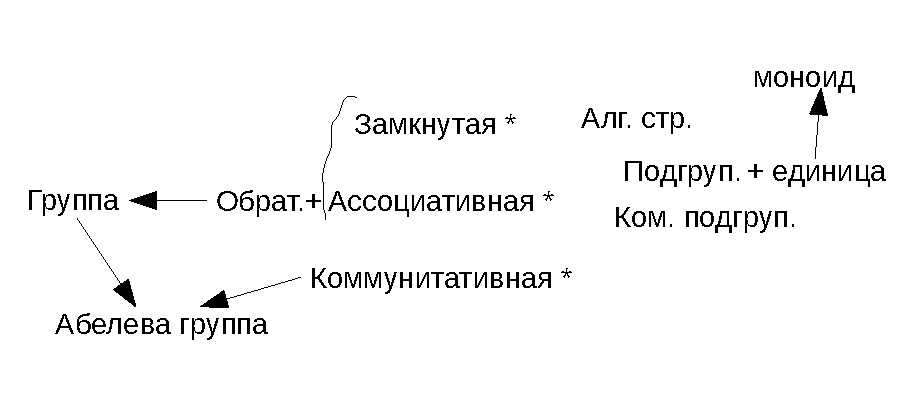
\includegraphics[]{./media/sv_group.pdf}

\begin{definition}[Кольцо]
	Кольцо - это мн-во в двумя операциями, связанными между собой дистрибутивными законами, если по одной из них оно является абелевой группой, по другому - полугруппой.
\end{definition}

\begin{remark}
	Операции в кольце условно наз-ся сложением и умножением, поэтому говорят об аддитивной группе и мультипликативной полугруппе кольца.
\end{remark}

\begin{remark}
	Если операция умножения в кольце обладает нейтральным элементом, то говорят, что это \textbf{кольцо с единицей}. Если операция умножения в кольце коммунитативна, то кольцо наз-ся \textbf{коммутативным}. 
\end{remark}

\textbf{Пример 1.}

\[ (M_n, +, \cdot) \]

Абелева группа по сложению, коммунитативна по сложения и т.д. Квадратные матрица образуют кольцо (некоммутативное, но с единицой).

\textbf{Пример 2.}

\[ (\mathbb{Z}, +, \cdot) \]

Кольцо, коммунитативное, с единицей.

\textbf{Пример 3.}

\[ (P[x], +, \cdot) \]

Кольцо многочленов.

\begin{definition}
	Множество $A = (K, +, \cdot)$ - поле, если на нём определены две бинарные операции: условно называемые сложение и умножение, удовлетворяющие следующим условиям:
	\begin{itemize}
		\item $(K, +)$ - абелева группа относительно сложения (с нейтральным элементом $\Theta$)
		\item $(K, \cdot), K^* = K \backslash \{\Theta\}$ - абелева группа относительно сложения (с нейтральным элементом $e$)
		\item Верен закон дистрибутивности $\forall a, b, c \in K:$
		\[
		\begin{aligned}
		(a+b)c = ac + bc \\
		a(b+c) = ab + ac
		\end{aligned}
		\]
	\end{itemize}
\end{definition}

\begin{remark}
	Каждое поле - кольцо, но не каждое кольцо - поле.
\end{remark}

~

$\{0,1\}$ - самое маленько (двухэлементное) поле.

\[ \mathbb{N} \subset \mathbb{Z} \subset \mathbb{Q} \subset \mathbb{R} \subset \mathbb{C} \subset \mathbb{H} \]

$\mathbb{H}$ - квадранион. $\mathbb{H} = \{ a + bi + cj + dR | a, b, c, c \in R \}, i^2 = j^2 = R^2 = -1$. "x"\ - вектор.

\begin{table}[h]
	\begin{tabular}{|c|c|c|c|c|c|c|}
		\hline
		Алг. действие & $\mathbb{N}$      & Кольцо цел. чисел $\mathbb{Z}$ & $\mathbb{Q}$                                                                            & $\mathbb{R}$         & $\mathbb{C}$        & $\mathbb{H}$ \\ \hline
		$+$           & КП                & АГ                             & АГ                                                                                      & \multicolumn{2}{c|}{\multirow{2}{*}{Поля}} & АГ           \\ \cline{1-4} \cline{7-7} 
		$\cdot$       & моноид (КП с ед.) & КП с ед.                       & \begin{tabular}[c]{@{}c@{}}КП с ед.\\ $\mathbb{Q}^* \backslash \{0\}$ - АГ\end{tabular} & \multicolumn{2}{c|}{}                      & Группоид     \\ \hline
	\end{tabular}
\end{table}

\begin{itemize}
	\item КП - коммутативная полугруппа
	\item КП с ед. - коммутативная полугруппа с единицей
	\item АГ - абелева группа
\end{itemize}

\begin{align}
	\textbf{13.02.2020}
\end{align}

\subsection{Группа преобразований}

Пусть функции $f: A \to B$ и $g: B \to C$ таковы, что $E_f = D_g$.

\begin{definition}[Композиция]
	Композицией (суперпозицией) функций $f: A \to B$ и $g: B \to C$ наз-ся новая функция $f \circ g: A \to C$, для которой верно условие $\forall a \in D_f : f \circ f(a) = g (f(a))$.
\end{definition}

\begin{theorem}[Корректность определения]
	Компизиция функции $f: A \to B$ и $g: B \to C$ при $E_f = D_g$ явл-ся функцией.
\end{theorem}

$h$ - функция $\eq \forall X \in D_h: \begin{cases} h(x) = c_1 \\ h(x) = c_2 \end{cases} \Rightarrow c_1 = c_2$

$h = f \circ g, \forall x \in D_h: \begin{cases} f \circ g(x) = c_1 \\ f \circ g(x) = c_2 \end{cases} \Rightarrow \begin{cases} g(f(x)) = c_1 \\ g(f(x)) = c_2 \end{cases} \Rightarrow f, g - \text{функция} \Rightarrow c_1 = c_2$.

\[ f = g \eq \forall x \in D_f = D_g: f(x) = g(x) \]

\begin{definition}[Нейтральная функция]
	id(x) = x
\end{definition}

\textbf{Свойства композиции функций:}

\begin{enumerate}
	\item $f \circ g \ne g \circ f$
	\item $f \circ (g \circ h) = (f \circ g) \circ h$
	\item $\forall f: id \circ f = f \circ id = f$, если $id(x) = x, \forall x$
	\item Композциция сюръекций - сюръекция
	\item Композиция инъекций - инъекция
	\item $\exists f' : f \circ f' = f' \circ f = id \eq f$ - инъекция
\end{enumerate}

\begin{theorem}[О группе биективных преобразований]
	Биективные преобразования множества относительно действия композиции образуют группу.
\end{theorem}

\begin{definition}[Преобразование]
	Биективное отображение множества $A$ в себя называется преобразованием множества $A$.
	\[ G = \{ f_i: A \to A | f_i - \text{биекция} \} \]
	\[ (G, \circ) - \text{группа} \]
\end{definition}

\[ GL_n(P) = \{A_n | detA_n \ne 0\} \]

Пусть $A$ - конечное множество, то есть $|A| = n$, где $n$ - натуральное число. $A = \{1, 2, 3, \dots, n\}$.

\begin{definition}[Симметрическая группа]
	Группа биективная преобразований конечного множества называется симметрической группой. Обозначение: $S_n, |S_n| = n!$
\end{definition}

\begin{definition}[Подстановка]
	Подстановка - элемент $u$ из $S_n$, записанный в виде
	\[
	u =
	\begin{pmatrix}
		\alpha_1 & \alpha_2 & \dots & \alpha_n \\
		\beta_1 & \beta_2 & \dots & \beta_n
	\end{pmatrix}
	\]
	где $u(\alpha_i) = \beta_i, i = \overline{1,n}$.
\end{definition}

\begin{align}
	\textbf{12.03.2020}
\end{align}

\subsection{Подстановки}

\[ (S(\chi), \degree) \]
\[ |\chi| = n \Rightarrow S(\chi) = S_n \]

По сути - это группа перестановок биективного множества и, следовательно, $|S_n| = n!$.

\[ u = 
\begin{pmatrix}
	1 & 2 & \dots & n \\
	u(1) & u(2) & \dots & u(n)
\end{pmatrix}
\]

\[ \forall i: \alpha_i, \beta_i, \gamma_i \in \{1,\dots,n\} \]

\begin{exmp}
	Есть две подстановки:
	\[
	\begin{pmatrix}
		1 & 2 & 3 & 4 & 5 & 6 & 7 \\
		7 & 3 & 1 & 2 & 4 & 5 & 6
	\end{pmatrix}
	\begin{pmatrix}
		1 & 2 & 3 & 4 & 5 & 6 & 7 \\
		7 & 2 & 4 & 3 & 5 & 6 & 1
	\end{pmatrix}
	=
	\begin{pmatrix}
	1 & 2 & 3 & 4 & 5 & 6 & 7 \\
	1 & 4 & 7 & 2 & 3 & 5 & 6
	\end{pmatrix}
	\] 
\end{exmp}

\begin{exmp}[Транспозиция]
	\[
	\begin{pmatrix}
		1 & 2 & 3 & 4 & 5 & 6 & 7 \\
		1 & 2 & 4 & 3 & 5 & 6 & 7
	\end{pmatrix}
	=
	(3,4)
	\]
\end{exmp}

\begin{definition}[Иденпотентный элемент]
	Элемент $u$ называется идентпотентным, если $u^2 = id$. Меняем 3 и 4 местами, опять меняем $\to$ они остались на своих местах $\to$ любой идентпотентный элемент является обратным самому себе.
\end{definition}

\[
	\begin{pmatrix}
		1 & 2 & 3 & 4 & 5 & 6 & 7 & 8 \\
		4 & 3 & 1 & 2 & 5 & 6 & 7 & 8
	\end{pmatrix}
	=
	(1, 4, 2, 3)
\]

\[ (1,2,3)^2 = (1,2,3)(1,2,3) = (1,3,2) \]
\[ r^3 = (1,3,2)(1,2,3) = (1)(2)(3) \]

Цикл $^2$ - всё осталось на месте, а 2-ка перешла в себя - тождественное преобразование.

\[ sign(u) =
\begin{cases}
	1, u - \text{чет.} \\
	-1, u - \text{нечёт.}
\end{cases}
\]

\section{Группы}

\begin{definition}[Нейтральный элемент]
	$e_1, e_2$ - нейтральные, $e_1 * e_2 = e_2 = e_1$
\end{definition}

$*$ - обратима, если:
\[ \forall a, b \in A \exists x, y \in A: \]
\[
\begin{cases}
	a * x = b \\
	y * a = b
\end{cases}
\]



\newpage

\tableofcontents

\end{document} % конец документа